\section{Method}

In this section, we introduce LongFlow, a novel KV cache compression method designed to overcome the limitations of prior work. Our approach is built on three pillars: a lightweight design philosophy, a rigorous theoretical derivation, and a high-performance system implementation.

\subsection{A Lightweight Design Philosophy}
The design of LongFlow is guided by a lightweight philosophy, standing in stark contrast to the conventional "look-back" approach of many prior methods. These methods assume that an accurate importance estimation requires aggregating historical information. As previously analyzed, this inherent dependency on historical data leads to prohibitive computational and memory overheads.
To break from this costly paradigm, we built LongFlow upon two core principles:



\noindent\textbf{The Principle of Zero-History Estimation.}
Our central hypothesis is that the current query, $\mathbf{q_t}$ contains sufficient information to effectively estimate the importance of all historical tokens.
To validate this premise, we conduct a preliminary analysis of SnapKV \citep{snapkv}.
We evaluate its performance on the LongBench benchmark \citep{longbench} while reducing the size of its query observation window. The results in Figure \ref{fig:snap} in Appendix show that the performance of SnapKV degrades only slightly as the query window gets smaller, which empirically demonstrates its remarkable robustness.
This evidence highlights the validity of the single-query method for importance estimation, forming the empirical foundation for our lightweight design.


\noindent\textbf{The Principle of Zero-Cost Estimation}
The second principle guiding LongFlow's design is Zero-Cost Estimation. This principle posits that the compression mechanism should not be an expensive, standalone process, but rather an intrinsic and nearly-free byproduct of the main attention computation. This stands in contrast to prior methods that often treat the importance estimation as a distinct step performed after the attention calculation.
Our method implements this principle by deriving the importance metric directly from an intermediate value of the standard attention forward pass which allows us to reuse the values that must be computed for the attention output. 
The reuse eliminates the need for auxiliary storage and ensures that the compression step adds no overhead.



\subsection{Derivation of the Importance Metric}
Our derivation of the importance metric begins with a formal definition of the eviction objective. Ideally, at any given step, we should evict the token whose removal has the minimal impact on the final logits across all future generation steps. This globally optimal objective is computationally intractable. To form a tractable objective, we first simplify our goal to minimizing the impact on the immediate next step's attention output, \( \mathbf{o}_{t+1} \):
\begin{equation}
\label{eq:next_step_objective}
\underset{i}{\arg\min} \left\| \mathbf{o}_{t+1} - \mathbf{o}_{t+1}^{(\setminus i)} \right\|^2,
\end{equation}
where \( \mathbf{o}_{t+1}^{(\setminus i)} \) is the new attention output computed without the key-value pair of token \( t_i \).

Although this objective is greatly simpler, it is still an unrealizable objective as it depends on the future query \( \mathbf{q}_{t+1} \).
Fortunately, we find a good approximation for this objective.
In our preliminary exploration, we find that the adjacent queries (\(\mathbf{q}_t, \mathbf{q}_{t+1}\)) have a high similarity (see Figure \ref{fig:cosine_sim} in Appendix, similar observation can be found in \citet{calidrop}). Intuitively, since the attention output is a weighted sum of Value vectors driven by the attention scores \( \mathbf{q}^T \mathbf{k} \), the strong similarity between adjacent queries implies that the overall attention distribution will be stable. This stability suggests that the impact of evicting a token at step $t$ is an excellent proxy for its impact at step $t+1$ if we omit the softmax denominator.
We thus formalize our practical approximation as follows:
\begin{equation}
\label{eq:greedy_objective}
\resizebox{\columnwidth}{!}{$
\left\| \mathbf{o}_{t+1} - \mathbf{o}_{t+1}^{(\setminus i)} \right\|^2 \approx \left\| \mathbf{o}_{t} - \mathbf{o}_{t}^{(\setminus i)} \right\|^2, \quad \text{where} \ i < t.
$}
\end{equation}
A formal error analysis of this approximation is presented in Section \ref{sec:error_bound_final}.

Directly computing this objective for all candidate tokens remains prohibitively expensive. To derive an efficient proxy, we analyze the structure of the attention output. The exact change in the output \( \mathbf{o}_t \) after evicting a historical token \( t_i \) is:
\begin{equation}
\label{eq:exact_change}
\resizebox{\columnwidth}{!}{$
\Delta \mathbf{o}_t = \mathbf{o}_t - \mathbf{o}_t^{(\setminus i)} = \sum_{j=0}^{t} \frac{\exp(s_t^j)}{Z} \mathbf{v}^j - \sum_{j \neq i} \frac{\exp(s_t^j)}{Z^{(\setminus i)}} \mathbf{v}^j,
$}
\end{equation}
where the unnormalized attention score of token $j$ is \( s_t^j = \mathbf{q}_t^T \mathbf{k}^j / \sqrt{d_k} \), and \( Z = \sum_{l=0}^{t} \exp(s_t^l) \) and \( Z^{(\setminus i)} = \sum_{l \neq i} \exp(s_t^l) \) are the softmax denominators before and after the eviction.

The main complexity arises from the change in this denominator from \(Z\) to \(Z^{(\setminus i)}\).
A further approximation is to omit the impact of eviction on the softmax denominator, assuming \( Z \approx Z^{(\setminus i)} \). This is a simple and reasonable assumption when the number of tokens is large (we discuss the error bound of this approximation in Section \ref{sec:error_bound_final}).
Under this approximation, the change in the output simplifies dramatically to the contribution vector of the evicted token itself:
\begin{equation}
\label{eq:approximated_change}
\begin{split}
\Delta \mathbf{o}_t 
&\approx \sum_{j=0}^{t} \frac{\exp(s_t^j)}{Z} \mathbf{v}^j - \sum_{j \neq i} \frac{\exp(s_t^j)}{Z} \mathbf{v}^j \\
&= \frac{\exp(s_t^i)}{Z} \mathbf{v}^i = \alpha_t^i \mathbf{v}^i,
\end{split}
\end{equation}

where \( \alpha_t^i \) is the attention weight of token $i$.

Thus, the objective is simplified to finding the minimum \( \alpha_t^i \mathbf{v}^i \).
We define the final importance score using the following equation for its computational simplicity and empirical effectiveness:
\begin{equation}
\label{eq:longflow_score}
\text{LongFlowScore}(t_i) = \left\| \alpha_t^i \mathbf{v}^i \right\|_1 =  \alpha_t^i \sum_{l=1}^{d} | (\mathbf{v}^i)_l |.
\end{equation}

The token with the minimum LongFlowScore is selected for eviction.
This method is exceptionally efficient. The contribution vectors \( \mathbf{c}_t^i = \alpha_t^i \mathbf{v}^i \) are a necessary intermediate result in the standard attention computation. Therefore, calculating the LongFlow score only requires performing an additional, lightweight reduction operation on this existing intermediate tensor. This perfectly realizes our Zero-Cost Estimation principle.


\begin{figure*}[t]
\centering
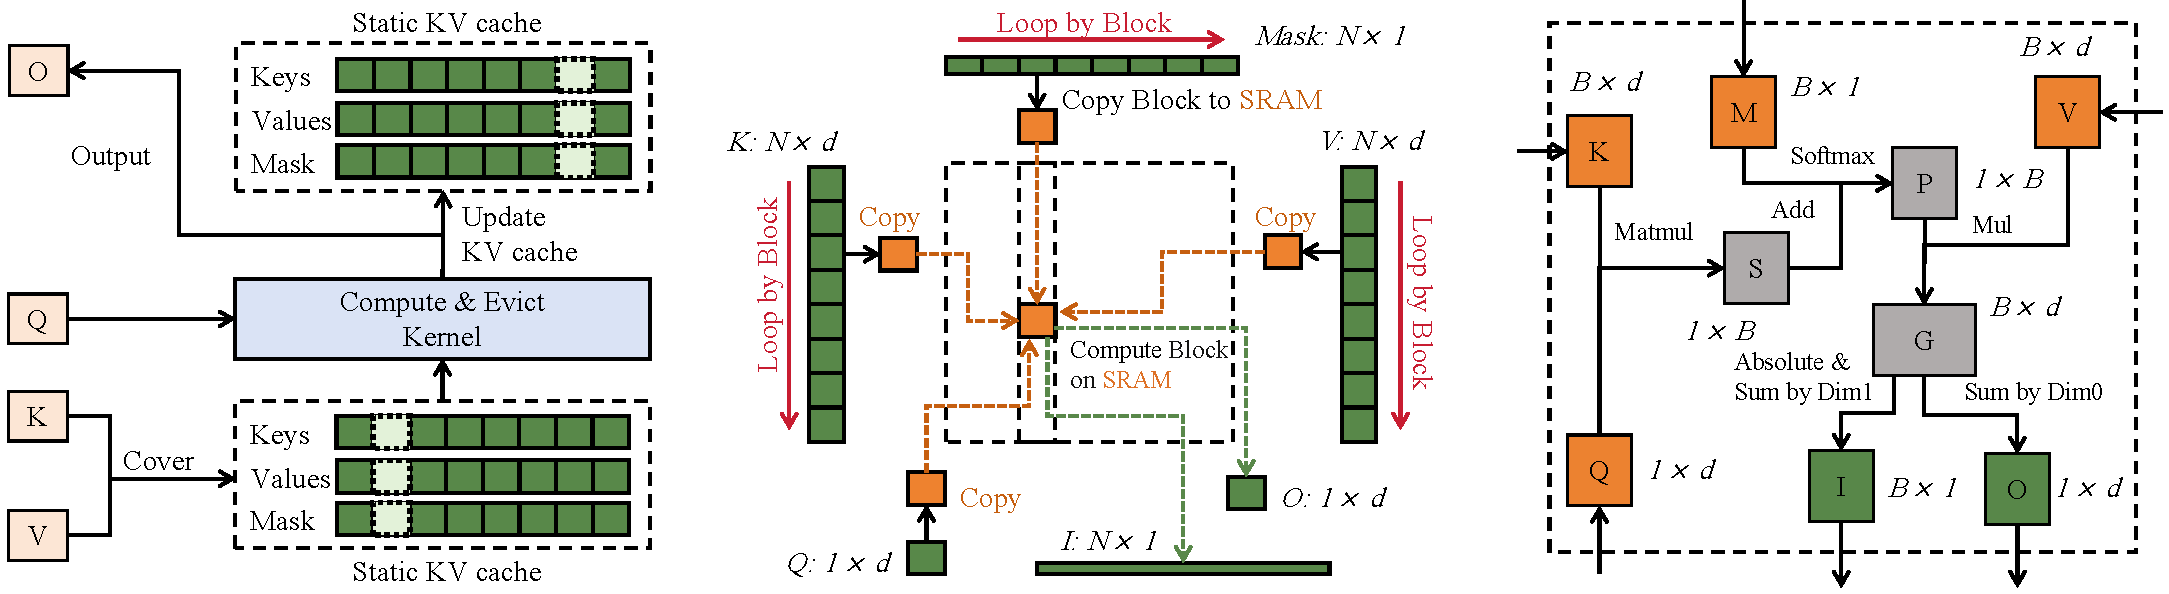
\includegraphics[width=0.95\linewidth]{figure/method_cropped.pdf}
\caption{The data and computation flow of our method. O: attention output; I: LongFlowScore; S, P and G are intermediate states in kernel forward pass. (\textbf{Left}): The process of a decoding step. The current KV will cover a slot selected in the previous step, and then the static KV and Mask will be sent to the kernel together with Q for calculation to obtain the current attention output and the slot to be covered in the next step. (\textbf{Middle}): The data flow between HBM and SRAM in the kernel. KV and Mask will enter SRAM by block and perform fused attention calculation. (\textbf{Right}): The computational flow on chip. Unlike standard flash attention calculations, we split the matrix multiplication of P and V into two steps and derive LongFlowScore from the intermediate result G.}
\label{fig:method}
\end{figure*}


%
%
%
%
%
%
%证明部分
\subsection{Theoretical Justification of the Approximations}
\label{sec:error_bound_final}

To derive the final LongFlow score from the ideal objective (from Equation \ref{eq:next_step_objective} to Equation \ref{eq:longflow_score}), we introduce two primary approximations: (1) using the contribution vector \( \mathbf{c}_t^i \) as a proxy for the true attention output change \( \Delta\mathbf{o}_t \) (the \emph{denominator approximation}), and (2) using the current query \( \mathbf{q}_t \) as a proxy for the next-step query \( \mathbf{q}_{t+1} \) (the \emph{query approximation}). We now provide a brief analysis of the error bounds for each. The detailed proofs are available in Appendix \ref{app:full_error_bound}.


The total error \( \mathcal{E}_i \) for a given token \( t_i \) is the difference between the ideal next-step objective and our practical score's squared magnitude:
\begin{equation}
\mathcal{E}_i = \left| \left\| \mathbf{o}_{t+1} - \mathbf{o}_{t+1}^{(\setminus i)} \right\|^2 - \left\| \alpha_{t}^i\mathbf{v}_i \right\|^2 \right|.
\end{equation}
Using the triangle inequality, we can decompose this error into two distinct sources:
\begin{equation}
\resizebox{\columnwidth}{!}{$
\mathcal{E}_i \le \underbrace{\left| \left\| \mathbf{o}_{t+1} - \mathbf{o}_{t+1}^{(\setminus i)} \right\|^2 - \left\| \mathbf{c}_{t+1}^i \right\|^2 \right|}_{\text{Error from Denominator Approx.}} + \underbrace{\left| \left\| \mathbf{c}_{t+1}^i \right\|^2 - \left\| \mathbf{c}_{t}^i \right\|^2 \right|}_{\text{Error from Query Drift}}.
$}
\end{equation}


\noindent\textbf{Error from the Denominator Approximation.}
This approximation replaces the true output change with the contribution vector of the evicted token. A rigorous algebraic manipulation shows that the remainder term of this approximation, \( \mathbf{R}_{t+1}^i = \Delta\mathbf{o}_{t+1} - \mathbf{c}_{t+1}^i \), is bounded by \( \|\mathbf{R}_{t+1}^i\| \le \frac{2V\alpha_{t+1}^i}{1-\alpha_{t+1}^i} \), where \(V = \max_j\|\mathbf{v}^j\|\). This bound confirms that the approximation is highly accurate when the attention weight of the evicted token \( \alpha_t^i \) is small. Since our method is designed to evict tokens with low attention, this approximation is well-justified.

\noindent\textbf{Error from the Query Approximation.}
Query approximation uses the score computed with the current query as a proxy for the ideal score that would be computed with the future query, \( \mathbf{q}_{t+1} \). The error introduced by this temporal approximation originates from the difference in attention weights, \( |\alpha_{t+1}^i - \alpha_t^i| \).
Due to the Lipschitz continuity of the softmax function, the change in output weights is bounded by the maximum change in the input pre-softmax scores, \(s_t^j\):
\begin{equation}
|\alpha_{t+1}^i - \alpha_t^i| \le \max_j |s_{t+1}^j - s_t^j|.
\end{equation}
The error in the scores, \( \Delta s^j = s_{t+1}^j - s_t^j \), arises from the query shift. By the Cauchy-Schwarz inequality, this error is bounded by \( |\Delta s^j| \le \frac{\|\mathbf{q}_{t+1} - \mathbf{q}_t\| \cdot \|\mathbf{k}^j\|}{\sqrt{d_k}} \). Assuming queries are normalized to unit vectors, we can relate the query difference to their cosine similarity: \( \|\mathbf{q}_{t+1} - \mathbf{q}_t\|^2 = 2(1 - \text{cos}(\mathbf{q}_t, \mathbf{q}_{t+1})) \). This gives a final bound on the maximum score error:
\begin{equation}
\label{eq:score_error_bound_final}
\max_j |\Delta s^j| \le \frac{\sqrt{2(1 - \text{cos}(\mathbf{q}_t, \mathbf{q}_{t+1}))} \cdot \max_j\|\mathbf{k}^j\|}{\sqrt{d_k}}.
\end{equation}
This bound provides a strong theoretical guarantee. It shows that as the similarity between consecutive queries approaches 1, the error from our temporal approximation approaches 0.


%
%
%
%
%
%
%
%
%
%
\subsection{High-Performance Implementation}



To realize the theoretical efficiency of LongFlow as practical speedups, we implement a high-performance system centered around a custom fused kernel.
This section details our key system-level optimizations, including the memory management strategy and the fused attention \& eviction kernel. Figure \ref{fig:method} shows the data and computation flow of our method.

\noindent\textbf{Static Memory and Consistent Workload.}
As established in our design philosophy, we employ a static KV cache and a consistent per-step eviction policy. The entire memory for the KV cache is pre-allocated to eliminate dynamic allocation overheads and memory fragmentation. By overwriting a single token at every decoding step, we ensure a consistent computational workload, which is particularly beneficial in distributed systems, as it guarantees a balanced workload and predictable overhead across all parallel workers.

\noindent\textbf{Fused Attention and Eviction Kernel.}
The core of our implementation is a custom Triton kernel that fuses the entire attention and eviction process. While our kernel is designed based on the I/O-aware principles of FlashAttention \citep{dao2022flashattention}, it incorporates three critical modifications to specifically and efficiently handle the auto-regressive decoding process with LongFlow:
(1) Given that the query sequence length is always 1 during decoding, we eliminate the outer loop over the query dimension in standard FlashAttention.
(2) To seamlessly integrate the online calculation of the LongFlowScore, we omit the running maximum used for numerical stability in safe softmax. To compensate and prevent potential overflow, we perform the calculation of softmax in FP32.
(3) We restructure the computation to maximize data reuse for both tasks. Within the single loop over KV cache blocks, we compute the un-normalized contribution vectors $exp(scores)V$ as a key intermediate result. This tensor is then summed along the sequence dimension to update the final attention output accumulator, and its L1-norm is calculated to serve as the un-normalized LongFlowScore for that block.
These modifications result in a single, highly-optimized operator that computes both the attention output and the token to evict in one pass, as detailed in Algorithm \ref{alg:longflow_kernel} in Appendix.